%!TEX root = ../template.tex
%%%%%%%%%%%%%%%%%%%%%%%%%%%%%%%%%%%%%%%%%%%%%%%%%%%%%%%%%%%%%%%%%%%
%% chapter3.tex
%% UNIPD thesis document file
%%
%% Chapter with introduction
%%%%%%%%%%%%%%%%%%%%%%%%%%%%%%%%%%%%%%%%%%%%%%%%%%%%%%%%%%%%%%%%%%%

\typeout{NT FILE chapter3.tex}%

\chapter{Fondamenti Teorici}

\prependtographicspath{{Chapters/Figures/Covers/}}

\section{Sistemi embedded e IoT}

\subsection{Introduzione ai sistemi embedded}
\noindent

I sistemi embedded rappresentano dispositivi di elaborazione integrati in apparecchiature specifiche, progettati per svolgere compiti dedicati con risorse limitate, offrendo un’elevata efficienza e un basso consumo energetico rispetto ai sistemi di uso generico.

Per la loro efficienza e alla capacità di operare con risorse contenute, questi sistemi sono ideali per applicazioni che richiedono alte prestazioni e affidabilità, come l’elaborazione audio in tempo reale.

Queste apparecchiature si trovano in dispositivi di uso comune come gli altoparlanti portatili, che offrono riproduzione audio continua e stabile, e nelle smart TV, che gestiscono il suono e rispondono rapidamente ai comandi dell’utente. Anche i citofoni con videocamera integrata sfruttano i sistemi embedded per elaborare audio e video in tempo reale, permettendo una comunicazione immediata.

Nel contesto della ristorazione, piattaforme embedded come il Raspberry Pi offrono soluzioni economicamente vantaggiose per la gestione dei flussi audio in tempo reale, permettendo una configurazione multi-zona che si adatta in modo flessibile alle esigenze acustiche di ciascuna area del locale.

Grazie alla disponibilità di componenti come \gls{gpio} e \gls{dac}, il Raspberry Pi rappresenta una soluzione versatile e adatta a integrazioni con sensori e interfacce audio aggiuntive. \cite{magpi2020}

Infine, la capacità di elaborazione in tempo reale, infatti, consente al sistema di adattarsi immediatamente ai cambiamenti ambientali, mantenendo la qualità e la coerenza dell’audio trasmesso in tutte le aree del ristorante.

\newpage
\subsection{L'IoT in ambito ristorativo}
\noindent

L'\gls{iot} ha rivoluzionato il settore della ristorazione, permettendo ai dispositivi di interagire e scambiare dati in modo autonomo e continuo. In tali contesti, i dispositivi \gls{iot} vengono utilizzati per gestire tutto, dal servizio clienti al controllo dell'ambiente.

L'integrazione di sensori e dispositivi audio consente ai ristoranti di monitorare e regolare in tempo reale i livelli del suono, il rumore ambientale e le preferenze dei clienti. Ad esempio: la musica di sottofondo può essere regolata automaticamente in base ai dati in tempo reale, come il feedback dei clienti o i livelli di rumore.

Alcuni sistemi possono persino tracciare la durata dei prodotti, facilitando la gestione delle scadenze e garantendo che gli alimenti siano conservati in condizioni ottimali. Questa soluzione non solo assicura il rispetto delle normative sanitarie, ma riduce anche il rischio di contaminazione alimentare e sprechi. \cite{10593159}

L'implementazione di queste tecnologie non si limita a migliorare l'esperienza del cliente nei ristoranti, ma aumenta anche gli standard di sicurezza, permettendo un controllo continuo dell'ambiente e delle operazioni, rendendo così il ristorante più reattivo ed efficiente.
\subsection{Raspberry Pi come piattaforma per sistemi audio}
\noindent

Il Raspberry Pi è considerato una piattaforma ideale per i sistemi embedded audio grazie al suo costo contenuto, alla versatilità e alla sua sufficiente potenza di elaborazione. Nel contesto di questo progetto di tesi, il Raspberry Pi Zero 2W viene utilizzato come unità centrale per gestire i flussi audio e distribuirli ai dispositivi client presenti nei tavoli. Il sistema impiega Mopidy, un server di streaming basato su Python e la sua estensione Iris per i controlli frontend, consentendo la gestione in tempo reale, ad esempio, di playlist e volume.

L’integrazione del Raspberry Pi con \gls{dac} e \gls{gpio} forma un’architettura flessibile e scalabile, facilmente espandibile con sensori e interfacce audio aggiuntive. Grazie al supporto per il multitasking e alla capacità di elaborazione parallela, il Raspberry Pi rappresenta un candidato ideale per le applicazioni audio nei contesti ristorativi, dove la gestione simultanea di più canali è essenziale. \cite{raspberrypi_doc}

Infine, la compatibilità del Raspberry Pi con numerose librerie rende il sistema altamente personalizzabile e facilmente adattabile a diversi contesti applicativi.

\newpage
\section{Tecnologie di streaming audio}

\subsection{Panoramica delle tecnologie di streaming audio}
\noindent

Lo streaming audio permette la trasmissione di dati audio in tempo reale su una rete, consentendo la riproduzione immediata senza necessità di download. Questa tecnologia si basa su protocolli che gestiscono il flusso costante di pacchetti di dati tra server e client  per garantire una riproduzione fluida. Due dei protocolli più diffusi sono il \gls{rtsp} e l'\gls{hls}. 

\begin{itemize}
    \item Il \gls{rtsp} è un protocollo di controllo per la gestione di sessioni di streaming in tempo reale, come video e audio, tra server e client. Ideato per offrire un controllo preciso del flusso multimediale, 
                              consente comandi come play e pause che funzionano come un telecomando per la gestione remota dei contenuti. Questo protocollo è spesso utilizzato insieme a \gls{rtp}, 
                                    che si occupa del trasporto effettivo dei dati audio e video, garantendo una sincronizzazione accurata.
                                          \gls{rtsp} è ampiamente utilizzato nelle telecamere di sorveglianza \gls{ip} per inviare video in tempo reale alle postazioni di monitoraggio. Anche nei sistemi di videoconferenza, 
                                                come Zoom, l'\gls{rtsp} supporta il controllo e la sincronizzazione dei flussi, offrendo una comunicazione in tempo reale senza interruzioni. \cite{s17040846}
          
    \item L'\gls{hls}, è un protocollo sviluppato da Apple che trasmette contenuti audio e video segmentandoli in piccoli blocchi, adattando automaticamente la qualità dello streaming alla larghezza di banda disponibile. 
                              Questo approccio adattivo lo rende ideale per garantire una riproduzione fluida su reti variabili e su dispositivi di vario tipo, dai telefoni cellulari ai computer. 
                                    Utilizzando \gls{http}, l'\gls{hls} è inoltre altamente compatibile con la maggior parte dei sistemi e dei browser.
                                          Piattaforme di streaming come Netflix e YouTube utilizzano l'\gls{hls} per offrire video in qualità adattiva, consentendo agli utenti di continuare a guardare senza interruzioni anche in caso di connessione instabile. \cite{flussonic2024}
  \end{itemize}

Entrambi i protocolli sono essenziali per mantenere una trasmissione audio a bassa latenza e di alta qualità, particolarmente importante in scenari che richiedono la sincronizzazione di più flussi in zone diverse. 

\subsection{Mopidy: Architettura e caratteristiche}
\noindent

Mopidy è un servizio open-source sviluppato in Python, progettato per la gestione e la riproduzione di audio sia da sorgenti locali che online. Funziona come un server \gls{http}, consentendo agli utenti di controllare la musica attraverso interfacce web e dispositivi remoti collegati alla rete. Mopidy è ideale per contesti che richiedono lo streaming audio multi-room, offrendo una soluzione flessibile e personalizzabile per ambienti pubblici e privati. Il sistema supporta diverse interfacce frontend, come Iris, Mopster, Muse e può integrarsi con piattaforme come Spotify, SoundCloud e file system locali.

Un aspetto distintivo di Mopidy è la sua architettura modulare, che consente agli sviluppatori di estenderne le funzionalità attraverso un’ampia gamma di plugin. Questa modularità rende Mopidy altamente adattabile a varie applicazioni, dalle configurazioni audio domestiche agli ambienti commerciali dove l’audio deve essere trasmesso in più zone.

L’uso dell’architettura client-server di Mopidy è particolarmente adatto alla gestione di più flussi audio in rete. Ogni client può essere collegato a una serie di altoparlanti, mentre il server gestisce la riproduzione dei file audio. Mopidy è spesso associato a Snapcast, un sistema di sincronizzazione audio tra client, che garantisce che tutti i dispositivi riproducano il flusso audio in modo perfettamente sincronizzato e senza ritardi percepibili. Questo sistema consente un controllo preciso sulla riproduzione audio in più luoghi, risultando ideale per spazi pubblici come scuole, uffici o campus multi-edificio.

Il server Mopidy può essere controllato da remoto utilizzando una varietà di interfacce, consentendo agli utenti di gestire playlist, controllare il volume e programmare la riproduzione utilizzando interfacce basate sul web e in riga di comando. Questa flessibilità rende Mopidy una soluzione molto efficace per gli ambienti in cui l'audio deve essere gestito da una postazione centrale.

\section{Acustica nei ristoranti}

\subsection{L'importanza dell'ambiente acustico nei ristoranti}
\noindent

Uno degli elementi chiave che definiscono la qualità acustica di uno spazio è il \gls{rt60}, che misura il tempo necessario del suono per dissolversi in un determinato ambiente. Nei ristoranti, ad esempio, un riverbero elevato può compromettere la chiarezza di un discorso, costringendo i clienti ad alzare la voce, con conseguente aumento dei livelli di rumore. Pertanto, un tempo di riverberazione ben controllato consente una comunicazione più chiara, creando un ambiente più confortevole per il cliente.

\begin{figure}[H]
      \centering
      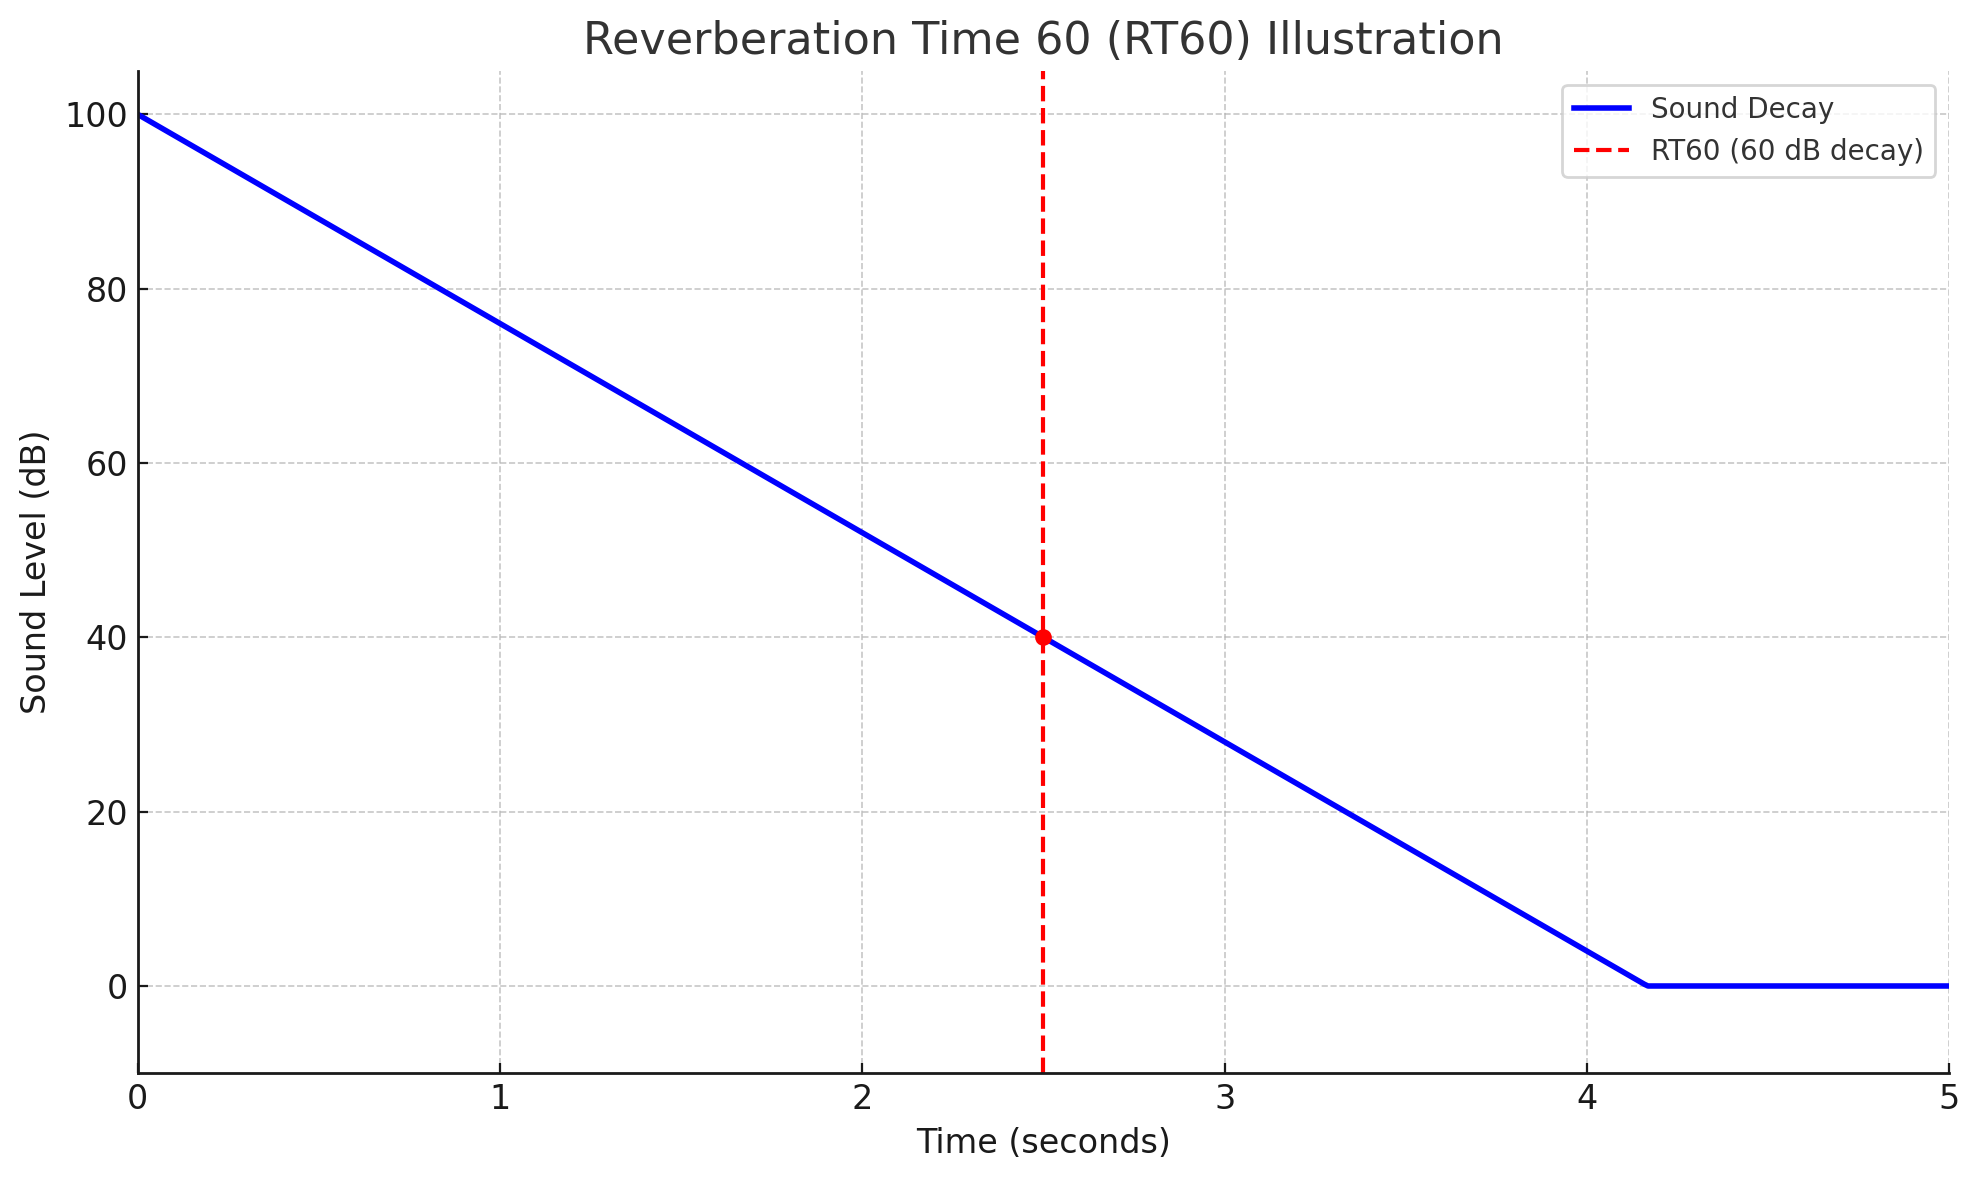
\includegraphics[width=0.6\textwidth]{Chapters/Figures/RT60.png}
      \caption{\small Diagramma del \gls{rt60} che mostra il decadimento del livello sonoro nel tempo in un ambiente. Il punto RT60, indicato dalla linea tratteggiata rossa, rappresenta il momento in cui il suono si riduce di 60 dB rispetto al livello iniziale.}
      \label{fig:RT60}
\end{figure}

Allo stesso modo, l'equilibrio tra assorbimento e riflessione del suono gioca un ruolo cruciale nel determinare il comfort acustico complessivo. Materiali come pannelli acustici, tappeti e imbottiture possono essere posizionati per ridurre la riflessione delle onde sonore. Quando le superfici sono molto riflettenti, creano echi e sovrapposizioni di onde sonore, che possono rendere l'ambiente caotico e sgradevole.

L'acustica e il comportamento umano sono correlati. Alti livelli di rumore nei ristoranti sono spesso associati a un aumento dello stress, a una riduzione del comfort e persino a una percezione negativa del cibo e del servizio. Alcuni studi hanno dimostrato che gli ambienti rumorosi possono portare a soggiorni più brevi e a un consumo più rapido dei pasti, in quanto i clienti possono trovare difficile rilassarsi. \cite{gbacoustics2023}

Inoltre, il livello di rumore può influenzare la percezione del gusto [\ref{cha:chapter4}], permettendo ai clienti di apprezzare maggiormente le sfumature di sapore e consistenza in ambienti acusticamente controllati. Al contrario, rumori eccessivi e un’atmosfera caotica possono compromettere queste percezioni, portando a un’esperienza meno piacevole.

Trovare il giusto equilibrio tra garantire il comfort acustico e creare un'atmosfera vivace è una delle sfide principali dell'acustica dei ristoranti. Molti locali moderni privilegiano spazi aperti, superfici dure e soffitti alti che, pur essendo esteticamente gradevoli, tendono ad amplificare il suono e ad esacerbare i livelli di rumore. Queste scelte progettuali possono determinare un ambiente acusticamente svantaggioso, soprattutto se combinato con un'alta densità di clienti. \cite{wiki:sound-restaurants}

\subsection{Il concetto di Bolle Sonore}
\noindent

Il concetto di "bolle sonore” si riferisce alla creazione di microambienti acustici personalizzati all'interno di uno spazio condiviso più ampio. In pratica, si tratta di progettare una configurazione audio in cui zone o aree diverse, come i singoli tavoli di un ristorante, possono avere paesaggi sonori isolati o personalizzati senza interferenze dai flussi audio circostanti. Le bolle sonore mirano a fornire un'esperienza uditiva mirata e coinvolgente per ogni ascoltatore o gruppo, migliorando la privacy e riducendo gli effetti negativi del rumore di fondo.

La creazione di bolle sonore richiede un preciso isolamento acustico e il controllo della distribuzione del suono. Questo può essere ottenuto attraverso una combinazione di barriere fisiche, altoparlanti direzionali e tecnologie di cancellazione del suono. I diffusori direzionali, ad esempio, concentrano i fasci audio in direzioni specifiche, impedendo al suono di diffondersi in altre aree. Allo stesso modo, i pannelli acustici o i divisori possono aiutare a bloccare le onde sonore dal passaggio oltre le zone designate.

In molti casi, la tecnologia utilizzata per creare bolle sonore coinvolge sistemi audio multi-room. Questi sistemi consentono di trasmettere flussi audio diversi alle varie parti di uno spazio, permettendo a ogni zona di avere un ambiente sonoro indipendente. Il sistema garantisce che ogni zona riceva il contenuto audio desiderato senza interferenze dalle zone adiacenti.

Snapcast, ad esempio, è un software molto diffuso che consente lo streaming audio sincronizzato su più dispositivi. Garantisce che tutti i client audio riproducano lo stesso flusso senza ritardi, rendendolo ideale per gli ambienti in cui la tempistica e il coordinamento sono fondamentali. In combinazione con Mopidy, che funge da server audio, Snapcast può trasmettere flussi audio distinti ad aree separate, creando bolle sonore controllate.

Oltre alle soluzioni basate sul software, l'hardware, come gli altoparlanti direzionali, può focalizzare il suono in direzioni specifiche, assicurando che solo il pubblico previsto lo senta chiaramente. Questi diffusori possono essere posizionati sopra o intorno a un'area specifica, ad esempio un tavolo da pranzo, per proiettare il suono direttamente nell'area di destinazione, riducendo al minimo la diffusione nelle zone adiacenti. Questa tecnologia è particolarmente utile negli ambienti open space, dove la gestione della dispersione sonora tra le zone è fondamentale.

Nelle applicazioni pratiche, le bolle sonore vengono utilizzate per creare ambienti audio personalizzati in spazi pubblici condivisi. Ad esempio, in un ristorante, ogni tavolo può avere un'esperienza sonora personalizzata, che si tratti di musica, conversazioni o altri contenuti audio. In questo modo i clienti possono godere di un'esperienza più intima e controllata, senza la distrazione di conversazioni vicine o rumori di fondo. 

Oltre che nei ristoranti, le bolle sonore trovano applicazione in vari spazi commerciali e pubblici, come musei, uffici e biblioteche, dove il controllo dell'ambiente uditivo è essenziale per migliorare l'esperienza degli utenti. Questi ambienti traggono vantaggio in quanto aiutano a bilanciare privacy, concentrazione e atmosfera senza ricorrere a un isolamento acustico completo. \cite{cit-multiaudio}

\begin{figure}[H]
      \centering
      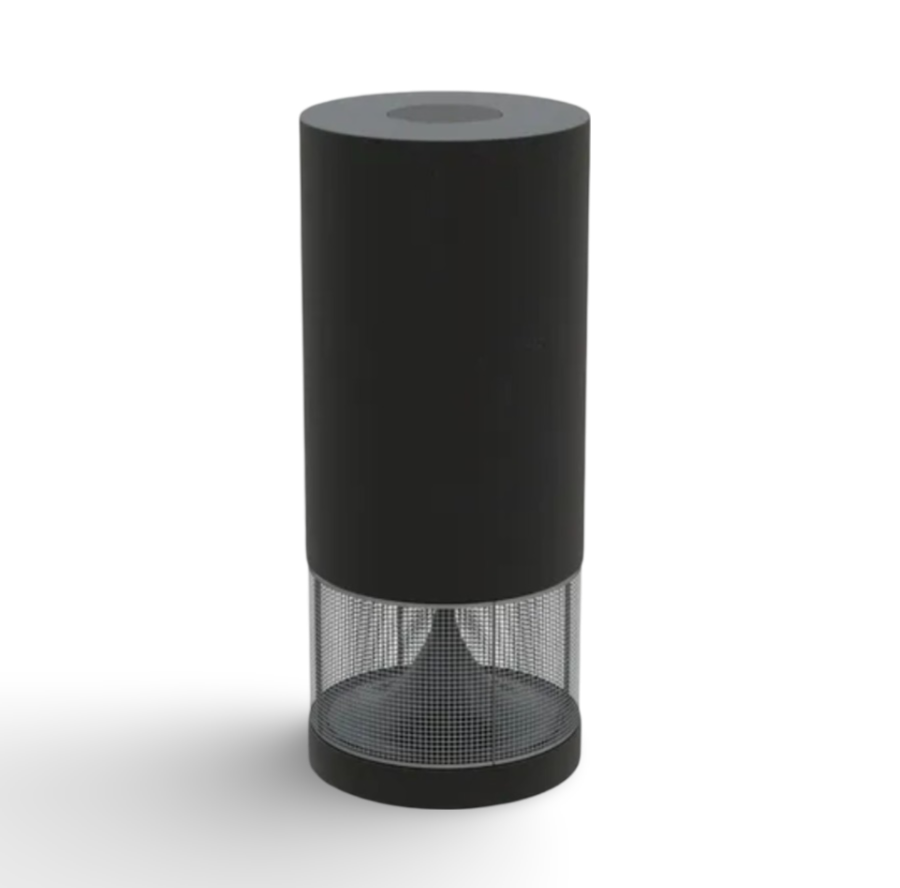
\includegraphics[width=0.5\textwidth]{Chapters/Figures/new_blender.png}
      \caption{\small Un modello 3D, progettato in Blender, del design degli altoparlanti direzionali. 
                        Ispirato ai design di Xiaomi. \cite{xiaomi2024}}
      \label{fig:blender_new}
\end{figure}